%!TEX TS-program = xelatex
%!TEX root = ../../maxwell2018thesis.tex

\chapter[The Complex Searcher Model]{The Complex Searcher Model}\label{chap:csm}
In this chapter, we present the~\gls{acr:csm}, an updated, conceptual searcher model that is one of the major contributions of this thesis. The~\gls{acr:csm} is an amalgamation and further development of prior, established searcher models. These models capture the complex sequence of interactions that take place between a searcher and a retrieval system. As such, this chapter provides a partial answer to our first high-level research question, \darkblueboxbold{HL-RQ1}.

\begin{figure}[h]
    \centering
    \vspace{4mm}
    \resizebox{1\hsize}{!}{
    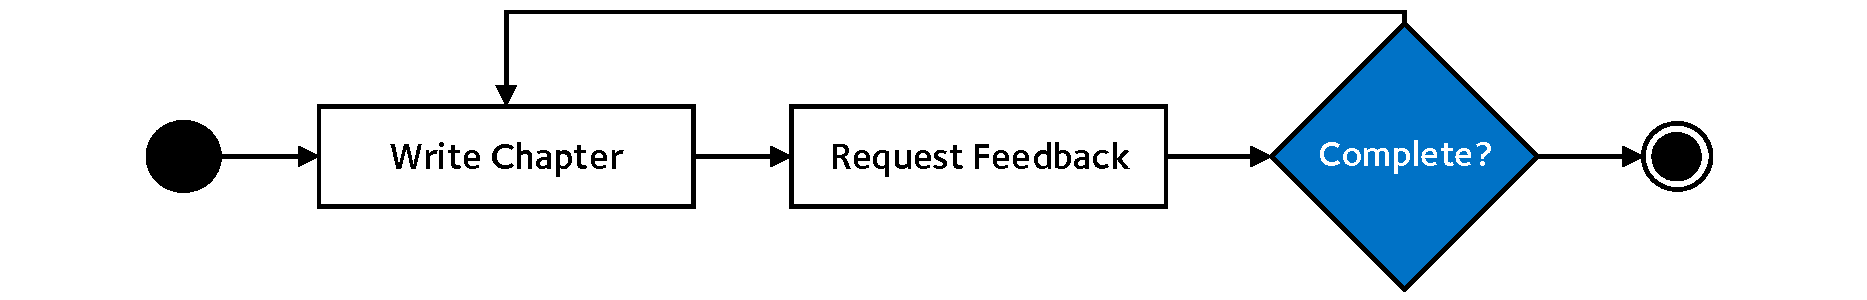
\includegraphics{figures/ch4-example.pdf}}
    \label{fig:model_example}
    \vspace{-5mm}
\end{figure}

As discussed in Section~\ref{sec:ir_background:user:models}, prime examples of prior searcher models include the Markov-based approach presented by~\cite{baskaya2013behavioural_factors}, and the model proposed by~\cite{thomas2014modelling_behaviour}. These searcher models (along with others) are in broad agreement with the general sequence of events that take place within the~\gls{acr:iir} process -- from issuing a query, to examining documents for relevance.

Given the aforementioned searcher models listed outlined in Section~\ref{sec:ir_background:user:models}, the~\gls{acr:csm} offers a number of advancements in modelling searcher and retrieval system interactions. In this chapter, we provide:

\begin{itemize}
    \item{the \emph{flow} of the proposed~\gls{acr:csm}, discussing the various steps and decisions that searchers subscribing to it undertake (Section~\ref{sec:csm:flow});}
    \item{a discussion of the \emph{stopping decision points} that the~\gls{acr:csm} considers (Section~\ref{sec:csm:stopping});}
    \item{a summary of the key advancements that the~\gls{acr:csm} provides (Section~\ref{sec:csm:advancements}); and}
    \item{an outline of the key \emph{assumptions} that we consider as part of the~\gls{acr:csm} (Section~\ref{sec:csm:assumptions}).}
\end{itemize}

We also briefly outline the specifics for evaluating the~\gls{acr:csm} as a viable searcher model (Section~\ref{sec:csm:evaluation}). Specific details of the implementation of the~\gls{acr:csm} are discussed in our general methodology chapter, Section~\ref{sec:method:simulation}. We begin this chapter however with a discussion of the flow of the~\gls{acr:csm}, discussing the different steps and decisions that searchers will make.

\section{Model Flow}\label{sec:csm:flow}
The~\gls{acr:csm} is illustrated as a flowchart in Figure~\ref{fig:csm}. It comprises as a number of different activities denoted by boxes, and decisions, represented as blue diamonds. The flowchart is divided up into a number of different blocks, labelled \blueboxbold{A} to \blueboxbold{F}. Each of these blocks denotes a logical set of interactions -- block \blueboxbold{B} for example considers all of the actions and decisions a searcher would undertake in relation to \emph{querying.} In this section, we outline the flow of the~\gls{acr:csm}, discussing the key activities and decisions that searchers would undertake. This is done in relation to the six labelled blocks.

\begin{itemize}
    
    \item[\blueboxbold{A}]{\blueboxbold{Topic Examination} A searcher subscribing to the~\gls{acr:csm} would begin the search process with some new information need. This would typically be provided as a \emph{topic,} with a topic description outlining said information need, and stating explicitly what would constitute a relevant document.}

\end{itemize}

\begin{figure}[t!]
    \centering
    \resizebox{1\hsize}{!}{
    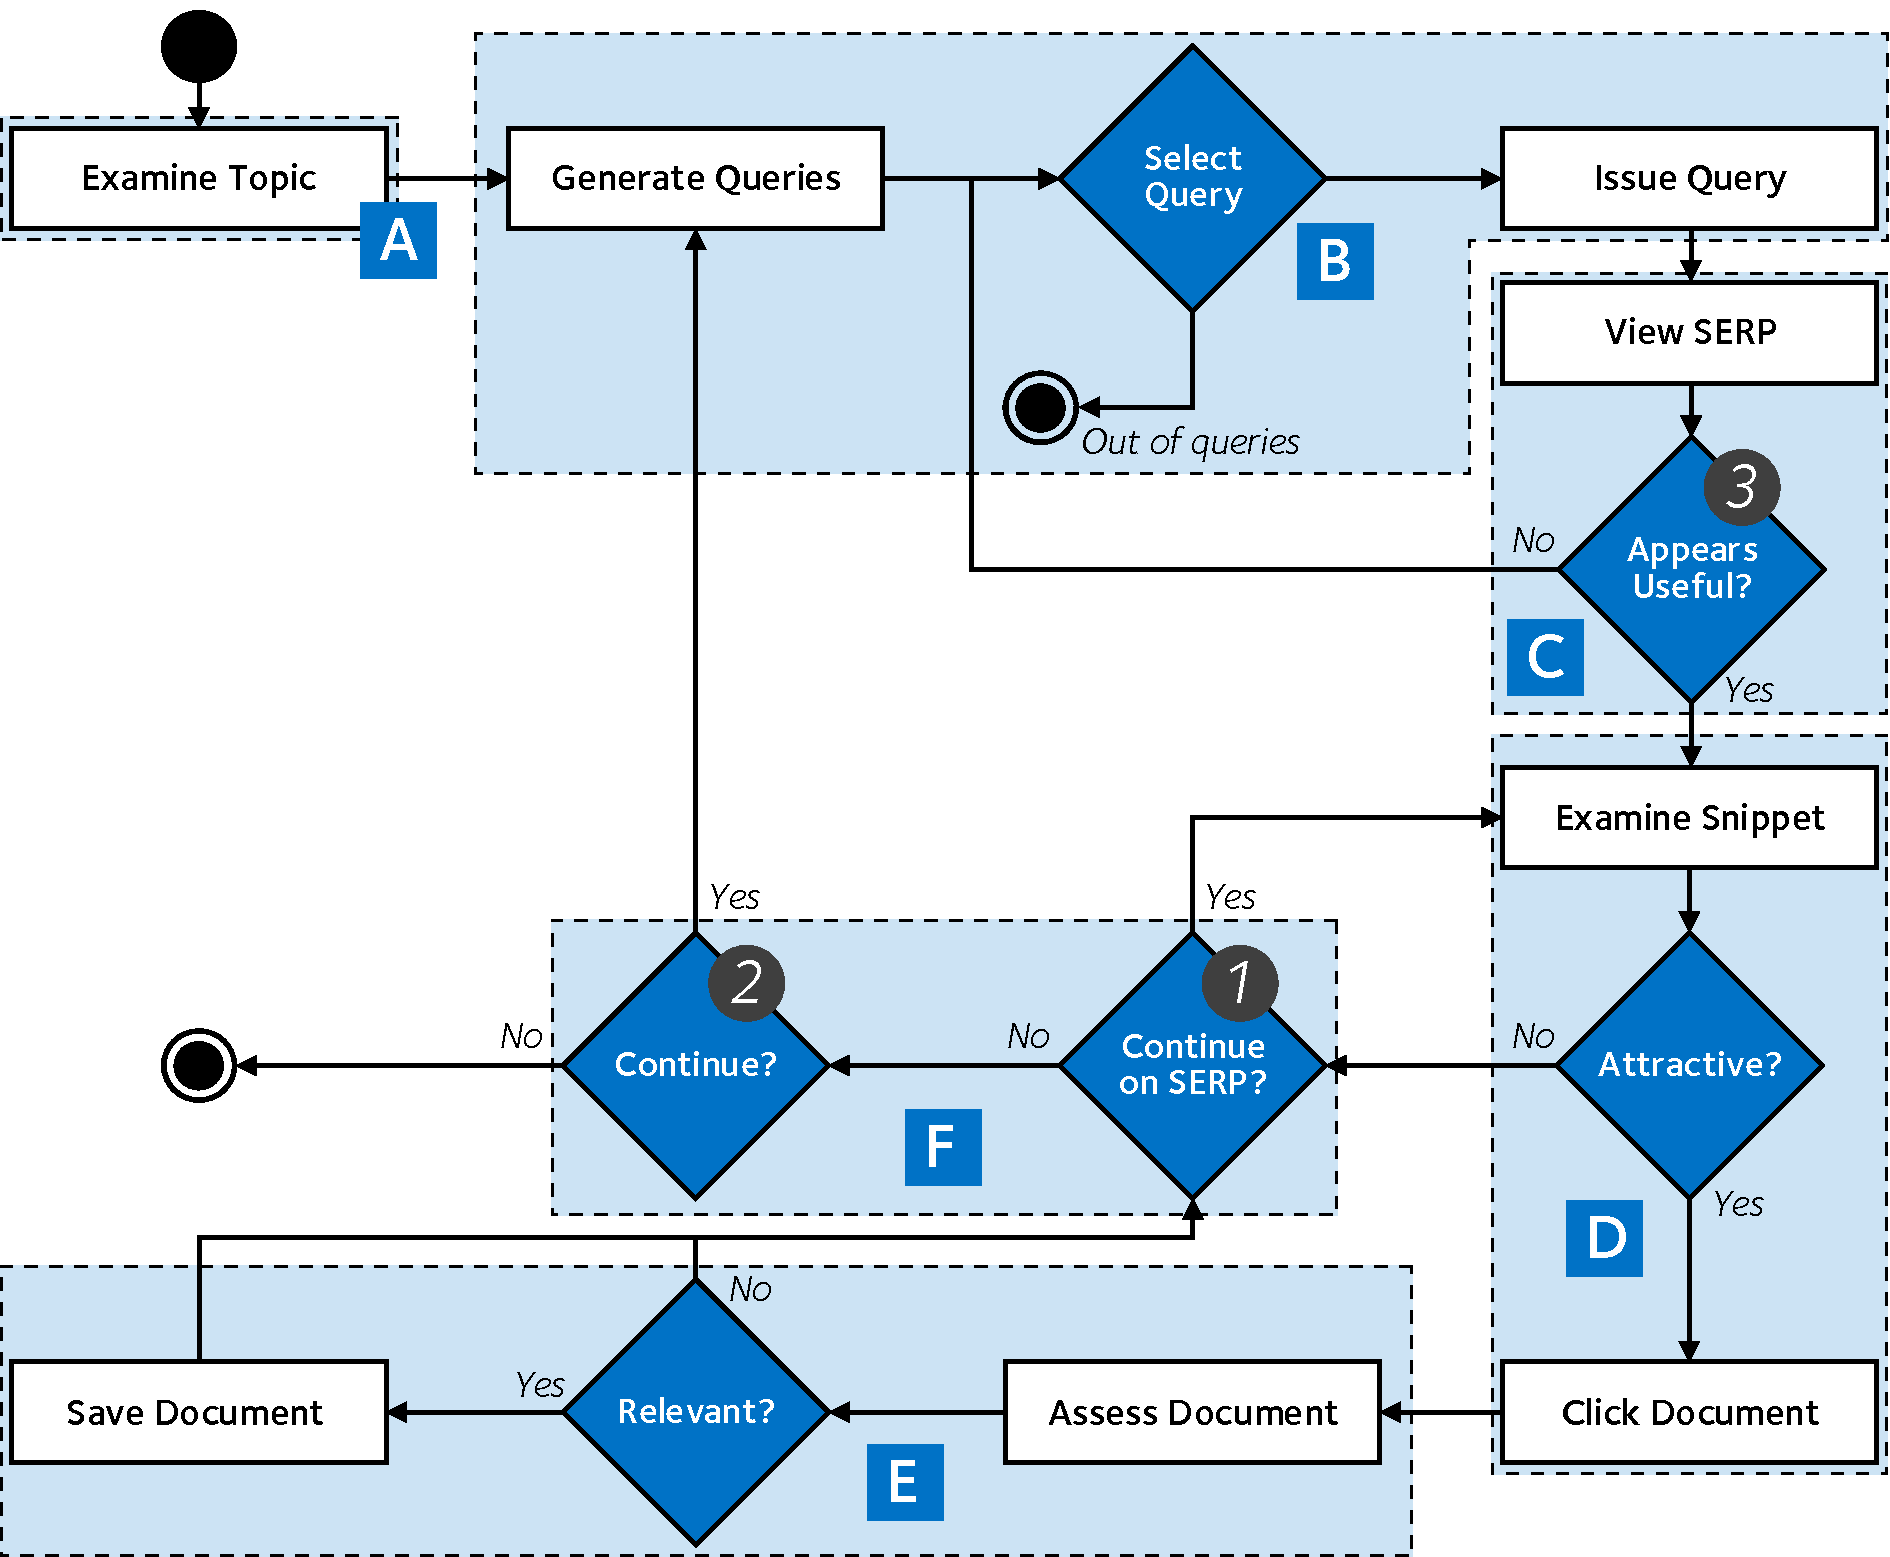
\includegraphics{figures/ch4-csm.pdf}}
    \caption[Flowchart of the~\gls{acr:csm}]{A flowchart of the proposed~\glsfirst{acr:csm}, as used in experimental work discussed later in this thesis. Main components as discussed in Section~\ref{sec:csm:flow} are labelled \blueboxbold{A} to \blueboxbold{F}, complete with light blue surrounding boxes. The \emph{three} stopping decision points are highlighted with \emph{1}, \emph{2} and \emph{3} (refer to Section~\ref{sec:csm:stopping}).}
    \label{fig:csm}
\end{figure}

\begin{itemize}
    
    \item[\blueboxbold{B}]{\blueboxbold{Querying} Once the information need has been established, the searcher will then move onto the \emph{querying} block. Here, a number of different activities and a decision point are considered in relation to querying. The first activity that the searcher will undertake is the \blueboxbold{generation of queries}. Given the information need, a searcher will then begin to formulate a number of \emph{candidate queries} that they could issue to the underlying retrieval system. This is achieved through the use of some form of \emph{querying strategy} that generates said candidate queries. The searcher then must make a decision as to what query they should issue. A query is \blueboxbold{selected} from the candidate queries list via some process (e.g. some form of ranking). This query is the one the searcher believes is most likely to return relevant documents. The query is then \blueboxbold{issued} to the underlying retrieval system\footnote{We assume that a searcher will have already selected a retrieval system to use beforehand, as discussed in Section~\ref{sec:csm:assumptions:tool}.}, with the searcher proceeding to block \blueboxbold{C}.
    
    As stated previously,~\gls{acr:iir} is an iterative process where multiple queries can be issued in a single search session. The~\gls{acr:csm} provides support for this -- as can be seen from the flowchart line from block \blueboxbold{F} to the querying block \blueboxbold{B}. At each point, the list of candidate queries queries generated could theoretically be regenerated, thus supporting query reformulation. If a searcher then finds that the candidate queries list has been exhausted, a stopping point is provided for this scenario.}
        
    \item[\blueboxbold{C}]{\blueboxbold{\gls{acr:serp} Examination} With the query now issued, the retrieval system will return to the searcher a~\gls{acr:serp}. From here, the searcher is able to \blueboxbold{view the~\gls{acr:serp}} -- that is, to obtain an \emph{initial impression} of the~\gls{acr:serp} by examining the various \emph{proximal cues}~\citep{chi2001information_scent} presented to him or her. If the~\gls{acr:serp} does not appear to look good, or offers a poor \emph{information scent,} the searcher will abandon the~\gls{acr:serp} and proceed to issue a further query from the list of candidate queries as described in block \blueboxbold{B}. If the~\gls{acr:serp} however does look \blueboxbold{useful}, and could potentially yield relevant material, the searcher will then \emph{enter} the~\gls{acr:serp}, and proceed to examine individual result summaries in detail.}
    
    \item[\blueboxbold{D}]{\blueboxbold{Result Summary Examination} Result summaries are presented to the searcher within the~\gls{acr:serp}. Searchers can take individual result summaries in turn, examining the title and snippet text provided for \blueboxbold{attractiveness}. If deemed to be sufficiently attractive to warrant further examination, the searcher will then click on the provided link, which will take the searcher to the associated document. However, if deemed to be not attractive enough, the searcher will then move to block \blueboxbold{F}, where a decision must be made regarding whether to continue on the~\gls{acr:serp}, and if not, whether to continue with the search session.}
    
    \item[\blueboxbold{E}]{\blueboxbold{Document Examination} Once a searcher clicks on an attractive result summary, he or she will then be presented with the associated document. This document is then \blueboxbold{assessed} by the searcher for relevance, after which a further decision must be made. \emph{Is this document relevant to the information need?} If so, the document is \emph{saved,} meaning that it is added to a list of documents that have been identified by the searcher as relevant. The searcher then proceeds to block \blueboxbold{F}. If not considered relevant, the searcher then proceeds directly to block \blueboxbold{F}.}
    
    \item[\blueboxbold{F}]{\blueboxbold{Deciding to Stop} Regardless of how the searcher reaches this block (either from block \blueboxbold{D} or \blueboxbold{E}), a searcher here can make two key stopping decisions. The first considers whether he or she should remain on the present~\gls{acr:serp}. If this is decided to be the case, the searcher will then move to the next result summary presented within it, and begin to examine that for attractiveness. If it is decided not to remain on the~\gls{acr:serp}, the searcher will then move to a final decision -- \emph{should I stop this search session, or continue?} If the searcher decides to continue the search session, he or she will then move back to the query generation activity in block \blueboxbold{A}, beginning the cycle again. Otherwise, the session will be abandoned.}
    
\end{itemize}

Of particular interest to the work in this thesis are the \emph{stopping decision points}, as shown in blocks \blueboxbold{C} and \blueboxbold{F} of Figure~\ref{fig:csm}.

\section{Stopping Decision Points}\label{sec:csm:stopping}
Outlined previously in Section~\ref{sec:stopping_background:why:points}, established searcher models consider stopping from two key perspectives: \emph{result summary level stopping,} and \emph{session level stopping.} The two established stopping decision points are included within the~\gls{acr:csm}, and are labelled \emph{1} and \emph{2} in Figure~\ref{fig:csm} respectively. They are also briefly outlined below.

\begin{itemize}
    \item[\blueboxbold{1}]{\blueboxbold{Result Summary Level Stopping} This stopping decision point concerns the depth at which a searcher will stop examining a list of ranked results. After stopping at this point, the searcher can continue the search session by issuing a further query.}
    \item[\blueboxbold{2}]{\blueboxbold{Session Level Stopping} This second stopping decision point considers the point at which a searcher will stop their search session in its entirety.}
\end{itemize}

The~\gls{acr:csm} however includes a third, \emph{\gls{acr:serp} level stopping decision point,} highlighted as stopping decision point \emph{3} within block \blueboxbold{C} of Figure~\ref{fig:csm}.

\begin{itemize}
    \item[\blueboxbold{3}]{\blueboxbold{\gls{acr:serp} Level Stopping} With this new stopping decision point, a searcher can abandon a~\gls{acr:serp} before \emph{entering} it and examining result summaries in detail.}
\end{itemize}

This new stopping strategy permits searchers subscribing to the~\gls{acr:csm} to be more savvy with their interactions. By gauging the~\gls{acr:serp}, he or she can make an informed decision as to the quality of said~\gls{acr:serp} before making the decision to invest more time examining its contents, or simply cutting their losses and abandoning it -- for better or for worse. The new stopping decision point is one of the key advancements that the~\gls{acr:csm} provides, and is discussed in more detail in Section~\ref{sec:csm:advancements:stopping} below.

\section{Model Advancements}\label{sec:csm:advancements}
The~\gls{acr:csm} provides two novel advancements to modelling the interactions between a searcher and retrieval system. These are highlighted as blocks \blueboxbold{B} and \blueboxbold{C} in Figure~\ref{fig:csm}, and denote advancements to the \emph{querying} process, as well as the inclusion of the aforementioned third stopping decision point respectively. In this section, we discuss each in turn. While the querying advancements are novel, they are not the core focus of this work, and thus discussion of the new~\gls{acr:serp} level stopping decision point will be in more depth.

\subsection{SERP Level Stopping}\label{sec:csm:advancements:stopping}
This new stopping decision point -- illustrated in block \blueboxbold{C} of the~\gls{acr:csm} (Figure~\ref{fig:csm}) -- is motivated by the idea of the \emph{information scent} present on a given~\gls{acr:serp}, with the notion of information scent discussed previously in Section~\ref{sec:stopping_background:theoretical:ift:patch}. This section also introduced the concept of \emph{proximal cues}~\citep{chi2001information_scent}, cues that provide insights into whether the presented~\gls{acr:serp} will yield information that will aid the searcher in satisfying their underlying information need. This has been previously demonstrated in prior studies~\citep{wu2014information_scent, ong2017scent_behaviour, maxwell2017snippets}.

By operationalising information scent as the perceived performance of a given~\gls{acr:serp}, we argue that incorporating this additional examination and associated stopping decision point allows a searcher to obtain an \emph{impression} of the~\gls{acr:serp}, before deciding to \emph{enter} the~\gls{acr:serp} and examine content in detail, or \emph{abandon} the~\gls{acr:serp} and move to the next activity. The notion of forming an impression is similar to the summary impressions formed by searchers subscribing to the model defined by~\cite{thomas2014modelling_behaviour}, as detailed in Section~\ref{sec:ir_background:user:models}. In their model however, a searcher would not form an overview of the~\gls{acr:serp}, but rather an impression of each individual result summary. The impression can then be used as a means of gauging whether further examination would be necessary.

This new stopping decision point is analogous to the well-studied phenomenon of \emph{\gls{acr:serp} abandonment} in which limited interaction occurs with the searcher. This has been typically assumed to provide an indication of the searcher's \emph{dissatisfaction} with the presented results~\citep{dassarma2008serp_abandonment, chuklin2012serp_abandonment, kiseleva2015serp_fails}, or \emph{satisfaction} (through the concept of \emph{good abandonment})~\cite{loumakis2011image_smells, wu2014information_scent}. Thus, we provide, to the best of our knowledge, the first searcher model that incorporates a path for a searcher to leave a~\gls{acr:serp} that appears to be of poor quality (or a \emph{low scent}), or satisfies their information need outright.

\subsection{The Querying Process}\label{sec:csm:advancements:querying}
Search sessions are inherently interactive~\citep{ingwersen2005theturn}. During a session, a searcher's underlying mental model of a given information need can adapt, and is likely to change as he or she examines new content for relevance~\citep{borlund2003iir_model}. Searchers may therefore find more descriptive terms associated with the information need, and incorporate these terms in a subsequent query reformulation.

From block \blueboxbold{B} in Figure~\ref{fig:csm}, the querying process has been broken up into two distinct activities and decisions: \emph{query generation} and \emph{query selection.} A searcher subscribing to the model will have the capability of revising their generated query list at each query reformulation, thus supporting the concept of the dynamic information need. Updated terms can in theory be selected from newly examined documents and incorporated within the query generation process.

Query selection then determines what one of the generated queries are to be issued to the retrieval system. Of course, the potential exists whereby all generated queries have been exhausted. This scenario would thus provide a natural stopping point for the searcher, as included in Figure~\ref{fig:csm}.

\section{Model Assumptions}\label{sec:csm:assumptions}
When modelling a real-world phenomenon, a number of different assumptions are made about said phenomenon's exhibited behaviours~\cite{fishwick1995simulation}. The~\gls{acr:csm} is no exception from this rule, and we make a number of different assumptions about a searcher's behaviours and the presentation of the retrieval system's results. This section details five key assumptions that we consider as part of the~\gls{acr:csm}.

\subsection{Search Task}\label{sec:csm:assumptions:task}
In this thesis, we are interested in the wider~\gls{acr:iir} process, considering all of the activities and decisions that constitute such a process. Indeed, we are interested in more than a simple retrieval task, such as a simple informational lookup.

The~\gls{acr:csm} provides scope for the modelling of a variety of different \emph{interactive search tasks.} Examples of these include the aforementioned \emph{ad-hoc,} exploratory, and \emph{diversity tasks.} These tasks can be undertaken in different search \emph{domains,} such as informational (refer to Section~\ref{sec:ir_background:user:iir}) or patent searching. As discussed in Section~\ref{sec:intro:rqs}, we exclusively consider informational search in the domain of news. Tasks we consider include both ad-hoc and diversity, such that we can examine how behaviours vary under each task. This is because while the~\gls{acr:csm} is able to model other search tasks, the selected search tasks provide for more interesting task types to examine, and consider a greater depth of activities and decisions that would not otherwise be examined in more simplistic lookup tasks, for example.

% we are interested in IIR. Interested in more than one simple task, not just lookup.
%
% considers \emph{interactive search tasks.} Such as ad-hoc, exploratory, diversity, etc. Different types and domains of interactive search task can occur, such as informational and patent search, respectively. As discussed in Section~\ref{sec:intro:rqs}, we use informational search in the domain of news. In this thesis, we consider both ad-hoc and diversity studies, and how behaviours vary under these different types of task. This is not to say that the~\gls{acr:csm} does not or cannot model other search tasks, such a simple lookup, for example. Such tasks provides a more interesting task type to examine.

These tasks are interesting to examine for two key reasons:

\begin{itemize}
    \item{the search goals between each task vary; and}
    \item{it is not clear when \emph{enough information is enough.}}
\end{itemize}

These reasons will undoubtedly produce interesting results between the two tasks, with the second providing a strong motivation for examining stopping behaviours in particular. As the tasks are not simple lookups, a searcher will not stop once a single relevant page has been found. Instead, he or she will stop once \emph{enough}~\citep{zach2005enough_is_enough} information has been found to satisfy their goal.

\subsection{Retrieval System Tool Choice}\label{sec:csm:assumptions:tool}
The searcher model proposed by~\cite{thomas2014modelling_behaviour} provides those subscribing to it with a choice as to what retrieval system they should use. As discussed earlier, we assume with the~\gls{acr:csm} that a searcher uses a single retrieval system. Our focus is therefore with the interactions that take place with a single retrieval system.

Of course, the inclusion of such a decision point would be interesting to examine within the wider~\gls{acr:iir} process. Different retrieval systems will have benefits and drawbacks for particular domain types (e.g. a patent retrieval system would perform better for patent searching tasks). It would be interesting to examine this kind of \emph{tool switching behaviour,} and could be considered as a further stopping decision point, or \emph{retrieval system stopping.}

\subsection{Simple SERPs}
When considering the~\gls{acr:serp} presented to the searcher as a whole, we make three simplifying assumptions within the~\gls{acr:csm}. These are listed and detailed below.

\begin{itemize}
    
    \item{\blueboxbold{Ten Blue Links} Under the~\gls{acr:csm}, a~\gls{acr:serp} will consist of a set of result summaries, coined in~\gls{acr:ir} literature as the \emph{ten blue links.} Of course, we acknowledge that additional components are present in contemporary~\glsplural{acr:serp}, such as multimedia content in federated search~\citep{chen2012federated_search_click_model}.}
    
    \item{\blueboxbold{Linear Examination Order} Once a searcher has decided to examine a~\gls{acr:serp} in detail, the result summaries presented to the searcher will be examined in the order in which they appear. There is evidence to suggest that real-world searchers examine results from top to bottom, as demonstrated by~\cite{joachims2002click_model, joachims2005click_model}, for example. Click models, such as the \emph{cascade model}~\citep{craswell2008click_models}, have been developed that employ this assumption. Such approaches are subject to \emph{positional bias,} where the searcher trusts the results of the retrieval model, and assumes that the first result presented is the most relevant to their information need.}
    
    \item{\blueboxbold{No Explicit Pagination} The~\gls{acr:csm} also assumes that the~\gls{acr:serp} presented to a searcher is of a single page, and no pagination of results exists. This does simplify the modelling process, with pagination not considered in prior searcher models that consider the session as a whole.}
    
\end{itemize}

\subsection{Good and Bad SERP Abandonment}
The~\gls{acr:csm} provides a new~\gls{acr:serp} level stopping decision point. Associated literature considers the notion of bad~\gls{acr:serp} abandonment, where a searcher is dissatisfied with the presented results. More contemporary research has introduced the notion of good~\gls{acr:serp} abandonment~\citep{khabsa2016good_abandonment}, where a searcher satisfies his or her information need by examining the~\gls{acr:serp}, and thus requires no further interactions with it. This is more prevalent on small-screen devices, where an information card presented to the searcher on the~\gls{acr:serp} may provide all the information required to satisfy a simple lookup task, for example.

\begin{figure}[t!]
    \centering
    \resizebox{1\hsize}{!}{
    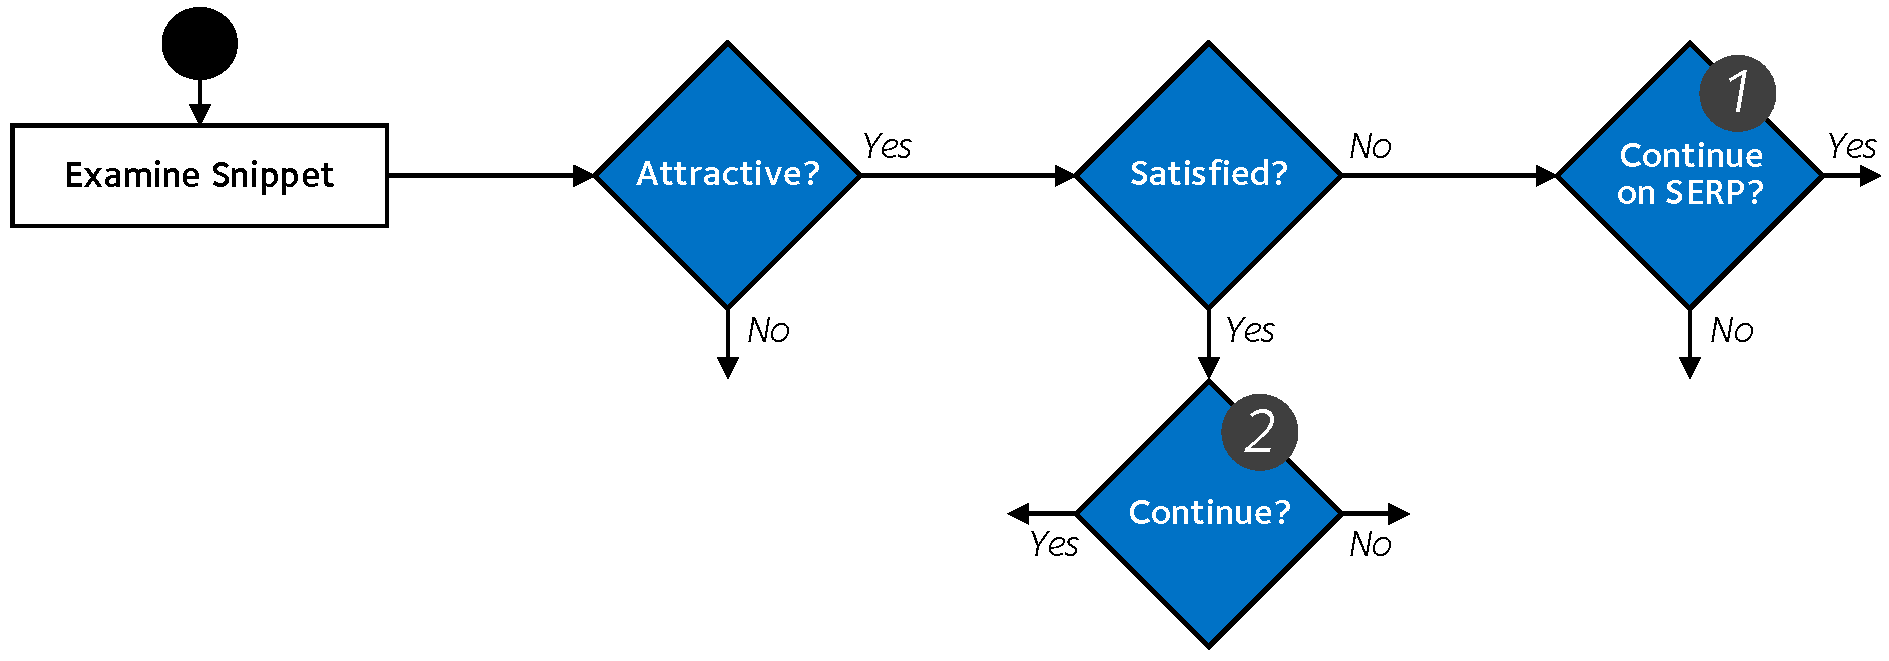
\includegraphics{figures/ch4-good.pdf}}
    \caption[Good abandonment flowchart]{An example of a process that can potentially provide for incorporating \emph{good~\gls{acr:serp} abandonment,} where a searcher satisfies his or her information need by simply examining a presented result summary. This is opposed to bad~\gls{acr:serp} abandonment, where the searcher will abandon a~\gls{acr:serp} if he or she feels the presented results are not of good quality.}
    \label{fig:good}
\end{figure}

The~\gls{acr:csm} does not explicitly consider the notion of good or bad~\gls{acr:serp} abandonment; the provision exists however for both to be modelled effectively within the scope of the new stopping decision point. Good abandonment can be for example catered for with the inclusion of an additional decision point after determining a result summary to be attractive; he or she could then make the decision to abandon the~\gls{acr:serp} if they feel satisfied with what they have examined. This is illustrated as an excerpt of a searcher model flowchart in Figure~\ref{fig:good}. The except demonstrates the result summary \emph{attractiveness} decision point, the additional decision point determining \emph{satisfaction} with what they have examined, and the final decision point that determines whether the searcher should abandon the~\gls{acr:serp}.

For the work in this thesis however, we assume a simple~\gls{acr:serp} consisting only of a ranked list of results. We also assume that searchers subscribing to the~\gls{acr:csm} will have complex information needs, as discussed in Section~\ref{sec:csm:assumptions:task} above. As such, we assume that the elements provided as part of the simplistic~\gls{acr:serp} are unlikely to fully satisfy their information need, and thus we consider~\gls{acr:serp} abandonment exclusively from the perspective of \emph{bad abandonment.} This is further discussed in Section~\ref{sec:csm:evaluation}.

\subsection{External Factors}
Given the flowchart of the~\gls{acr:csm} in Figure~\ref{fig:csm}, it is clear that the model is completely agnostic of \emph{external factors} that could potentially influence how an individual searches.~\cite{kelly2009iir} for example cited that:

\begin{quote}
    \emph{``searcher behavior [sic] can be governed by a number of external factors. For instance, the occurrences of a holiday or a project deadline will likely change the kinds of behaviors users exhibit and these behaviors may not represent their typical behaviors.''}
    \attrib{\cite{kelly2009iir}}
\end{quote}

These examples allude to time pressures, but there are a virtually unlimited number of other external reasons that may influence a searcher's behaviour. Even simple everyday occurrences such as a phone call or an incoming e-mail can sufficiently distract the searcher that their searching behaviours are altered. Our assumption is that the individual searches in a more controlled environment, where they are explicitly tasked to search.

\section{Evaluating the CSM}\label{sec:csm:evaluation}
The~\gls{acr:csm} is presented as a generalised, conceptual model of the search process. It captures the key activities and decisions that a searcher must undertake during the search process. Given the current searcher models presented in Section~\ref{sec:ir_background:user:models}, the~\gls{acr:csm} introduces further levels of complexity and realism into searcher models. Given our choice of search tasks and types and assumptions, three key assumptions are made for the evaluation of the model.

\begin{itemize}
    \item{\blueboxbold{Costs} We assume that a searcher will incur some cost when performing an individual activity within the~\gls{acr:csm}. For example, a document examination cost will be incurred when a searcher decides to examine a document for relevance.}
    \item{\blueboxbold{Bad Abandonment} As described previously, searchers in this thesis will only abandon a~\gls{acr:serp} if they consider it to be of poor quality. Given the complex information needs we consider in this work, this is a reasonable assumption to make.}
    \item{\blueboxbold{Gain} Following on from the above, searchers will only accrue gain for documents that they consider to be relevant to the given information need. We do not assume that a searcher will be able gain from examination of result summaries, for instance -- the information need is complex, and it is unlikely this will be done in practice.}
\end{itemize}

\section{Chapter Summary}
This chapter has proposed the~\glsfirst{acr:csm}, our solution to partially addressing \darkblueboxbold{HL-RQ1}. Building on prior searcher models, the~\gls{acr:csm} proposes different advancements to modelling a searcher's interactions, the main development being the inclusion of a new,~\gls{acr:serp} level stopping decision point. We have outlined a number of different assumptions that we make in the~\gls{acr:csm}, and also discussed some evaluation considerations related to the work in this thesis. Empirical work presented in Chapter~\ref{chap:csm} tests the~\gls{acr:csm}, providing evidence to support \darkblueboxbold{HL-RQ1} in that the~\gls{acr:csm} does provide improvements over the current searcher models.

In the next chapter, we turn our attention to some of the different stopping strategies that we operationalise -- and subsequently implement -- as part of the stopping decision points encoded within the~\gls{acr:csm}.

\newpage
\thispagestyle{empty}
\mbox{}